\documentclass[11pt,a4paper]{article}
\usepackage[margin=2.4cm]{geometry}
\usepackage{amsmath,amssymb}
\usepackage{tikz}
\usetikzlibrary{arrows.meta}
\usepackage{enumitem}
\setlength{\parskip}{5pt}\setlength{\parindent}{0pt}
\tikzset{a/.style={-{Stealth[length=2.4mm]},thick},v/.style={circle,draw,fill=black,inner sep=1.6pt}}

\begin{document}

{\large\bfseries Is it possible for 2-d kernels to improve Galvin's bound?}\\[2pt]

\medskip\hrule\medskip

\section*{Existing Result}

The Dinitz problem: an $n\times n$ grid, every cell gets its own list of $n$ colours. Can I always pick one colour per cell so that no row or column repeats a colour?

\begin{itemize}[leftmargin=1.4em]
    \item Draw arrows between cells in the same row or column (using a Latin square to decide directions). Every cell ends up with $n-1$ arrows going out.
    \item Lemma 1: if lists are bigger than the number of outgoing arrows, and every part of the graph has a \emph{kernel} (a set of cells that don't clash, where every other cell points into it), then colouring is possible.
    \item So lists of size $(n-1)+1=n$ are enough.
\end{itemize}

\textbf{The Idea:} use a 2-d kernel instead (every cell outside it points to \emph{two} cells inside). Then each colour I use would remove two arrows instead of one, and thus lists of about half the size would be enough.

\section*{Problem 1: the bound is already the smallest possible}

One row has $n$ cells and they all clash with each other. So they need $n$ different colours. If every list were $\{1,2,\dots,n-1\}$, I just don't have enough colours for one row.

So $n$ is not just an upper bound, it is the exact answer. Nothing smaller can be true, with any method. Same for any bipartite graph: all edges at one vertex touch each other, so I need at least (max degree) colours, and Galvin gives exactly that.

\section*{Problem 2: a row never has a 2-d kernel}

In the proof, each round picks a colour and looks at all cells that have that colour in their list. The lists can be anything, so those cells could be \textbf{exactly one row}.

\begin{center}
    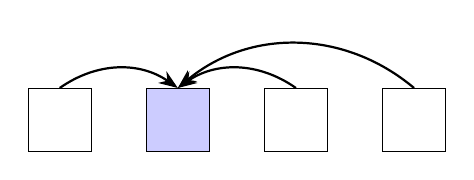
\begin{tikzpicture}
        \foreach \j in {0,1,2,3}{\node[draw,minimum size=0.8cm] (c\j) at (\j*1.5,0) {};}
        \node[draw,minimum size=0.8cm,fill=blue!20] at (c1) {};
        \draw[a] (c0.north) to[bend left=35] (c1.north);
        \draw[a] (c2.north) to[bend right=35] (c1.north);
        \draw[a] (c3.north) to[bend right=40] (c1.north);
    \end{tikzpicture}
\end{center}

\begin{itemize}[leftmargin=1.4em]
    \item All cells in a row clash, so I can only choose \textbf{one} cell (blue).
    \item Then each other cell can point to at most \textbf{one} chosen cell. A 2-d kernel needs two.
\end{itemize}

So no 2-d kernel, no matter how I draw the arrows. The proof breaks in the very first round. I checked it also breaks on just two cells with one arrow between them: neither cell can be outside the set (each has at most one arrow out), but both can't be inside (they clash).

\section*{Problem 3: I tried a softer version, it still fails}

I noticed the proof doesn't really need two arrows every time. With list size $\lceil d/2\rceil+1$ ($d$ = outgoing arrows), removing one arrow is enough when $d$ is odd:

\begin{center}
    \begin{tabular}{c|cccccc}
        $d$                  & 0 & 1 & 2 & 3 & 4 & 5 \\\hline
        $\lceil d/2\rceil+1$ & 1 & 2 & 2 & 3 & 3 & 4
    \end{tabular}
\end{center}

Going $3\to2$ lowers it, but $4\to3$ does not. So when $d$ is even, one arrow buys nothing.

\textbf{Where it gets stuck:} take a cell $u$ with the most outgoing arrows and keep an even number of the cells it points to.

\begin{center}
    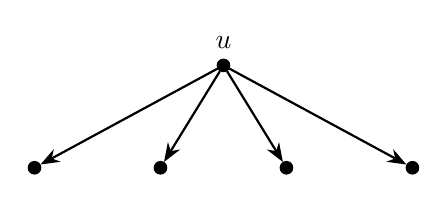
\begin{tikzpicture}
        \node[v,label=above:$u$] (u) at (0,1.3) {};
        \foreach \i/\x in {1/-2.4,2/-0.8,3/0.8,4/2.4}{\node[v] (v\i) at (\x,0) {}; \draw[a] (u)--(v\i);}
    \end{tikzpicture}
\end{center}

\begin{itemize}[leftmargin=1.4em]
    \item If I colour a bottom cell, $u$ loses a colour and one arrow, but $4\to3$ buys nothing.
    \item If I colour $u$, a bottom cell loses a colour and no arrow at all (the arrow points away from it).
\end{itemize}

So the process gets stuck on this piece, and it has about $d$ cells. Paying for a stuck piece of that size costs about $d$ extra colours, which is more than the $d/2$ I was trying to save. I checked this with code on all small graphs (up to 5 and 6 vertices) and it never beat the normal bound.

\section*{Things I got confused about}

\begin{itemize}[leftmargin=1.4em]
    \item I thought my arguments were about random digraphs and not the Dinitz grid. But a single row of the grid with Galvin's arrows is exactly one of those examples (all cells in a line, each pointing to the smaller ones). So it applies to Dinitz directly.
    \item Stuck does not mean the graph can't be coloured. The star above is easy to colour by hand. It only means \emph{this method} can't continue.
    \item Galvin's arrows are already the best possible for this kind of proof: in any arrow pattern that works, some cell in a row points to all the other $n-1$.
\end{itemize}

\section*{What I concluded}

\begin{enumerate}[leftmargin=1.4em]
    \item For Dinitz, the bound $n$ is exact. There is nothing to improve.
    \item 2-d kernels fail immediately on a single row.
    \item Even the relaxed version gets stuck on a star, and the cost of being stuck is bigger than the saving.
\end{enumerate}

\section*{Questions I want to ask}

\begin{itemize}[leftmargin=1.4em]
    \item Should I move to other graph classes where the bound is not already exact? I read that for perfect graphs many arrow patterns always have kernels (Boros and Gurvich). Could that give better bounds somewhere?
    \item Is a bound like $\lceil(\Delta+1+\omega)/2\rceil$ worth trying on a small class? I read it is an open conjecture in general (list version of Reed's conjecture).
    \item Do my 2-d kernel results (chordal graphs, acyclic digraphs, etc.) have a use somewhere else, even if not for colouring?
\end{itemize}

\end{document}